\section{首先，致敬伟人GKxx}

\begin{frame}{革命尚未成功，同志仍须努力}
    \begin{center}
        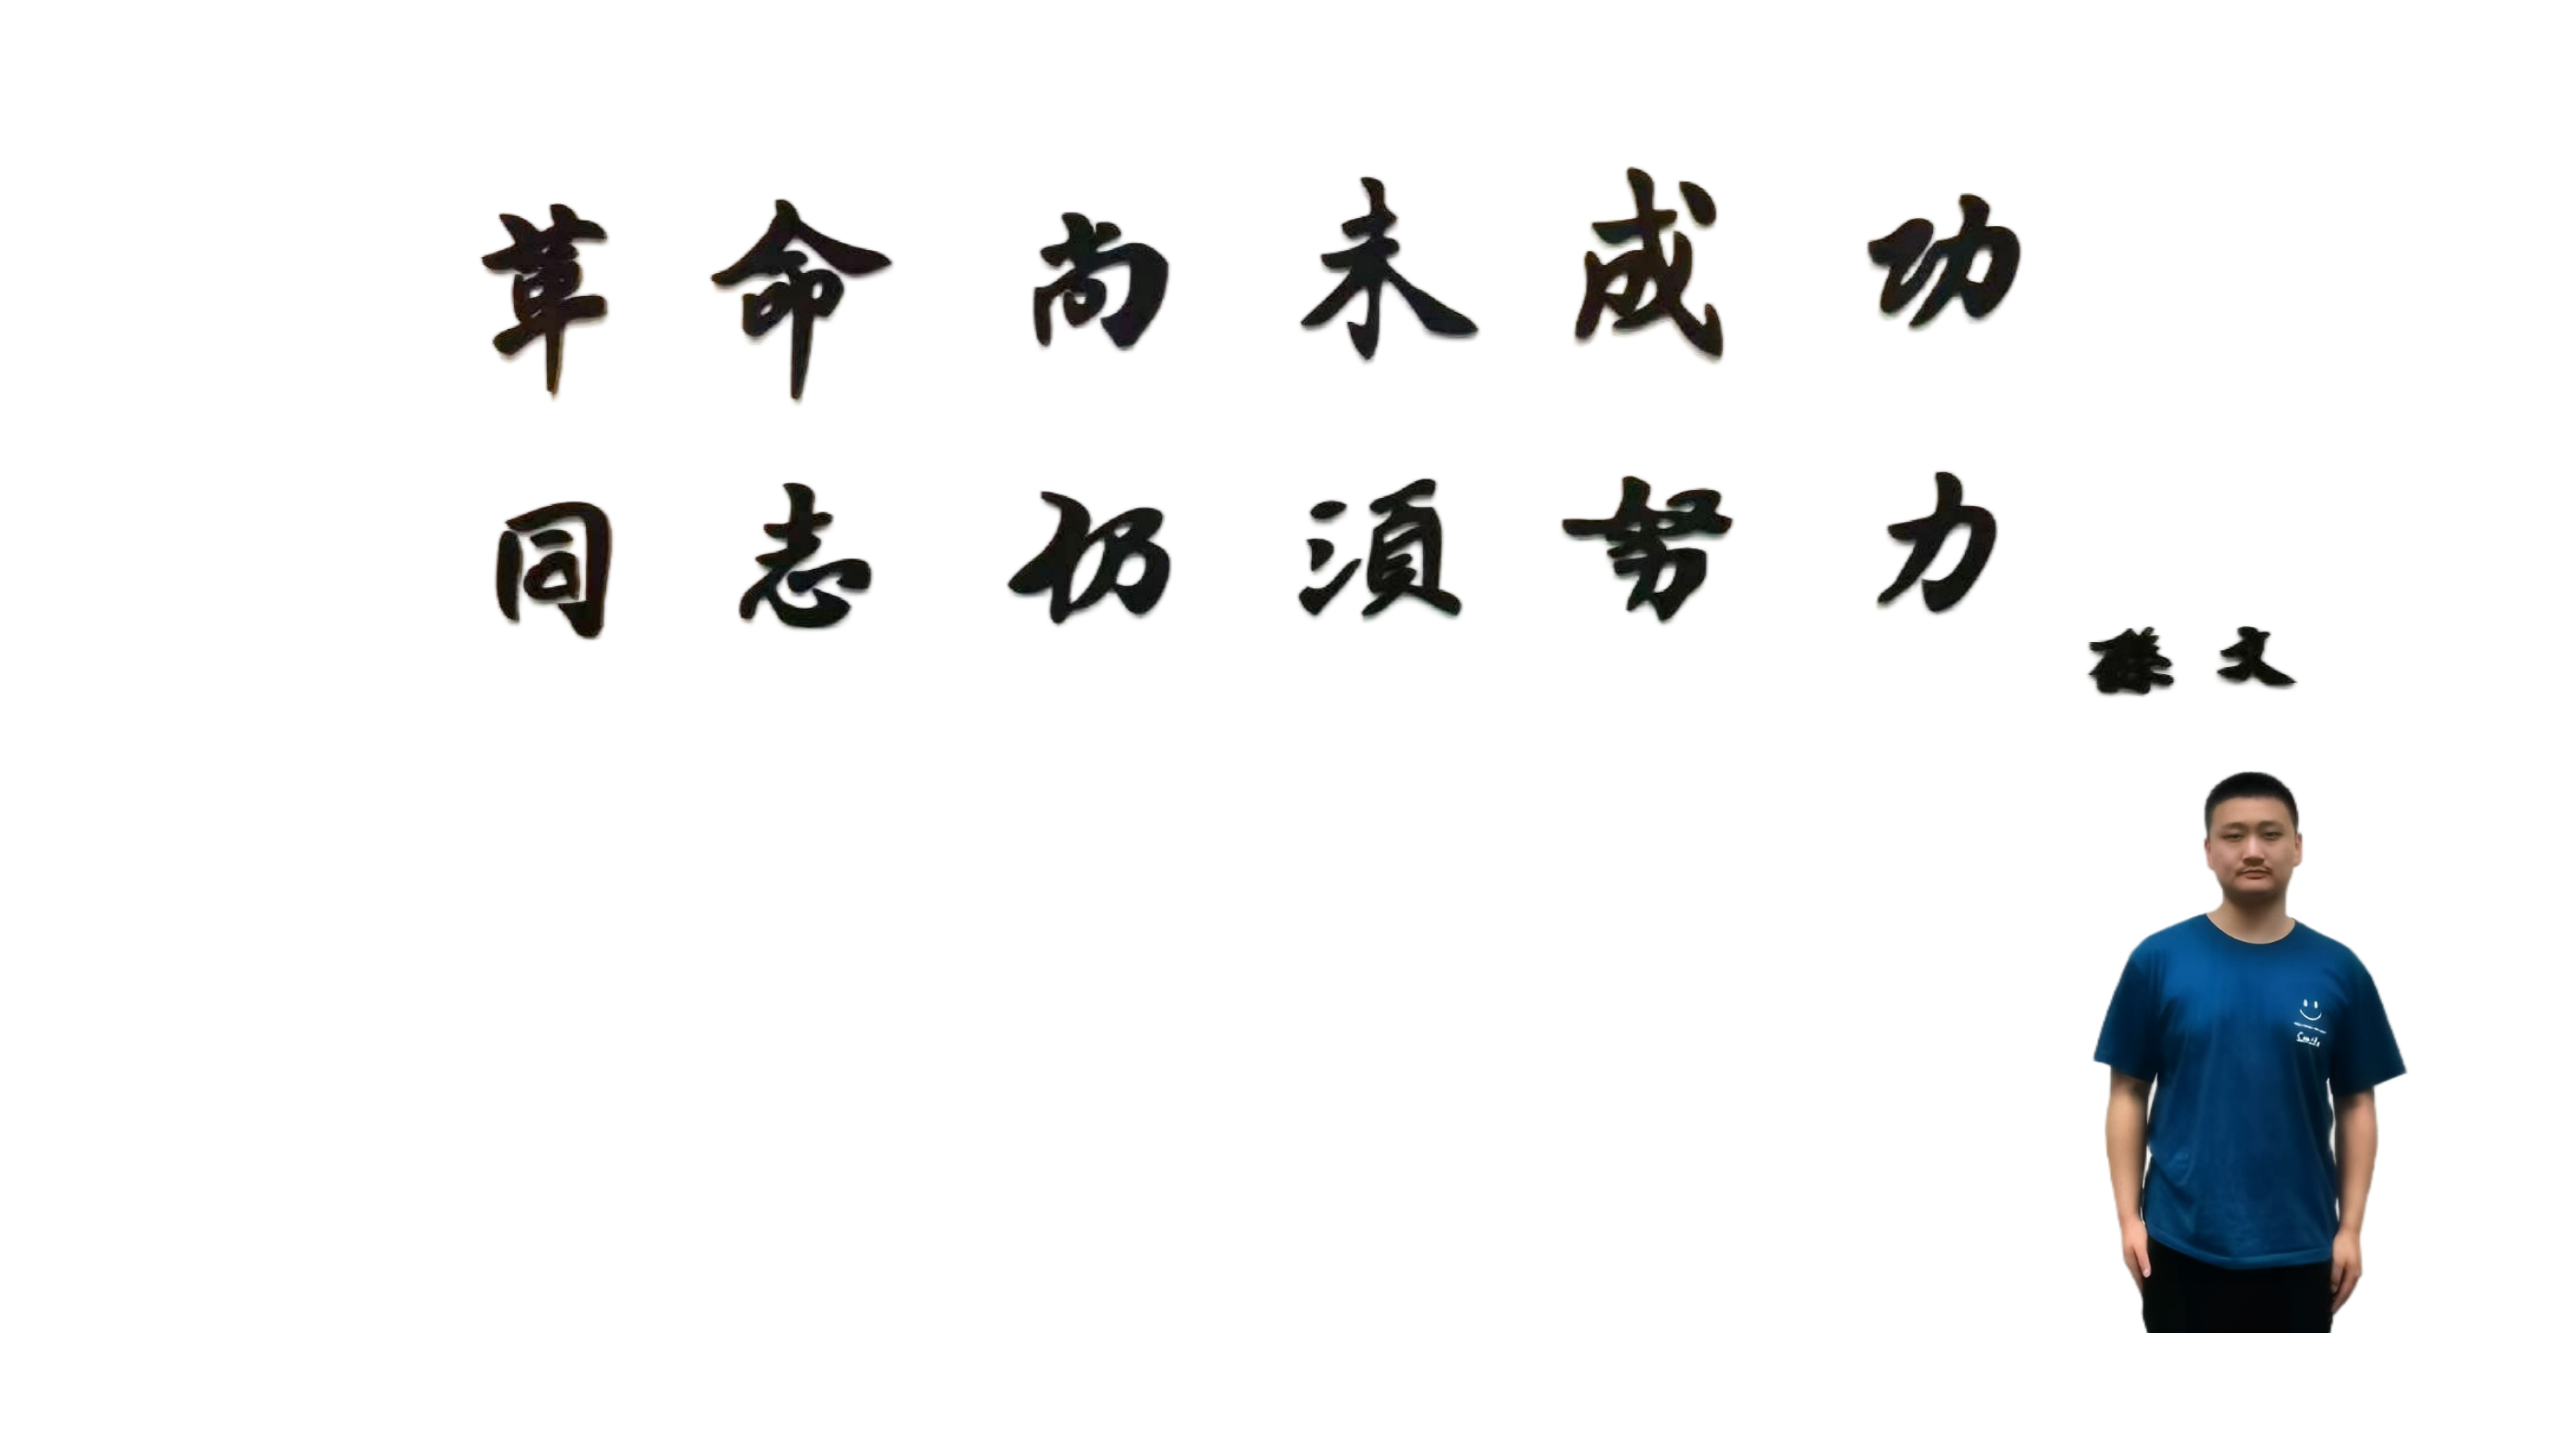
\includegraphics[width=\linewidth,height=0.72\textheight,keepaspectratio]{gkxx.png}
    \end{center}
\end{frame}

\begin{frame}{GKxx：现代CS100的重要建设者}
    GKxx是上海科技大学2020级计算机科学与技术专业学生，曾多次担任CS100的TA。

    \begin{itemize}
        \item 深度参与课程建设，推动课件内容与教学方式的改良。
        \item 改进课程考核，为我们今天的CS100打下了重要基础。
        \item 如今已经“飞升”国科大／中国科学院软件研究所。
    \end{itemize}

    \begin{vspquote}{致敬，也接力}
        今天的课程建立在前人的投入之上。把课讲清楚，把工具做好，把这份认真传下去。
    \end{vspquote}

    Bilibili：\textbf{GKxxISCAS}\qquad
    GitHub：\href{https://github.com/GKxxUCAS}{\textbf{GKxxUCAS}}
\end{frame}
